For this task, we used the NLTK library to calculate the number of unique tokens that exist in a review. Then, we plotted the graphs to show the distributions of the tokens, both with and without stemming.

We can see the figure below. Figure 2 shows the number of unique tokens without stemming in every review, while Figure 3 shows the number of unique tokens after stemming is performed in every review.

\begin{figure}
    \centering
    \caption{Distributions of tokens in each review (without stemming)}
    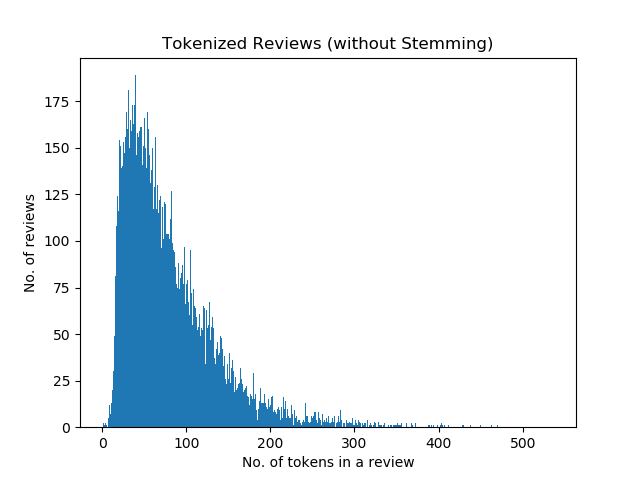
\includegraphics[scale=054]{figures/token_review.png}
    \label{fig:tokenized_review}
\end{figure}

\begin{figure}
    \centering
    \caption{Distributions of tokens in each review (with stemming)}
    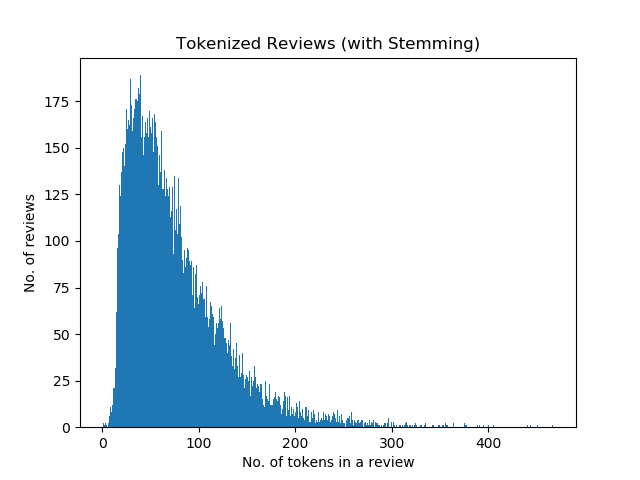
\includegraphics[scale=0.5]{figures/stem_review.png}
    \label{fig:stemmed_token_review}
\end{figure}

To make the comparison easier, in Figure 4, the stems are indicated with the color orange, while the tokens are indicated with the color blue.

Based on Figure 4, we can conclude that the number of unique tokens with stemming is generally lower that the number of unique tokens without performing stemming.

\begin{figure}
    \centering
    \caption{Comparison of the distributions of the tokens with and without stemming}
    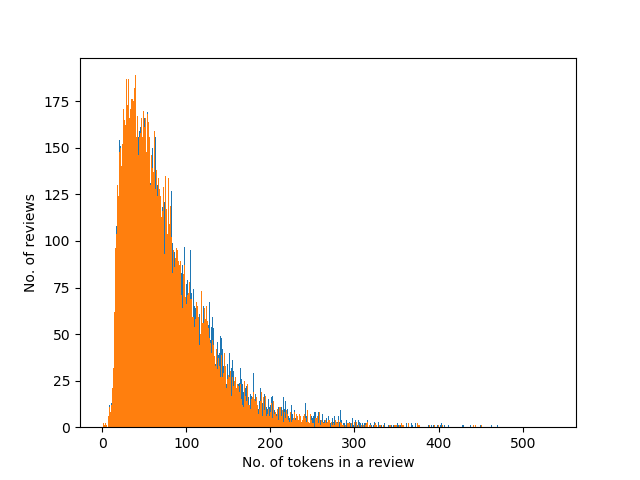
\includegraphics[scale=0.5]{figures/token_stem_review.png}
    \label{fig:stem_and_token_review}
\end{figure}

\begin{table}[]
    \centering
    \caption{20 most common unique tokens}
    \begin{tabular}{|c|c|c|}
        \hline
        No. & Token & No. of Appearances  \\
        \hline
        1 & food & 8580 \\
        2 & place & 8236 \\
        3 & good & 7919 \\
        4 & great & 6295 \\
        5 & service & 6027 \\
        6 & like & 5534 \\
        7 & get & 5216 \\
        8 & time & 5172 \\
        9 & would & 5168 \\
        10 & one & 5044 \\
        11 & back & 4717 \\
        12 & go & 4145 \\
        13 & really & 3731 \\
        14 & also & 3333 \\
        15 & got & 3171 \\
        16 & us & 2926 \\
        17 & even & 2891 \\
        18 & order & 2820 \\
        19 & could & 2815 \\
        20 & nice & 2756 \\
        \hline
    \end{tabular}
    \label{tab:most_common_tokens}
\end{table}

\begin{table}[]
    \centering
    \caption{20 most common unique stems}
    \begin{tabular}{|c|c|c|}
        \hline
        No. & Stem & No. of Appearances  \\
        \hline
        1 & place & 9407 \\
        2 & food & 8731 \\
        3 & good & 8055 \\
        4 & time & 6588 \\
        5 & get & 6390 \\
        6 & servic & 6338 \\
        7 & great & 6302 \\
        8 & like & 6231 \\
        9 & order & 6150 \\
        10 & go & 5993 \\
        11 & one & 5278 \\
        12 & would & 5168 \\
        13 & back & 4744 \\
        14 & tri & 3978 \\
        15 & come & 3784 \\
        16 & realli & 3731 \\
        17 & also & 3333 \\
        18 & love & 3291 \\
        19 & got & 3171 \\
        20 & even & 3160\\
        \hline
    \end{tabular}
    \label{tab:most_common_stems}
\end{table}